\begin{frame}
  \frametitle{\problemtitle}
  \begin{block}{Problem}
  	Given $\ell$ players on the left of a table and $r$ players on the right, how many different pairs face each other during a game of around-the-table?
  \end{block}
	  \centering
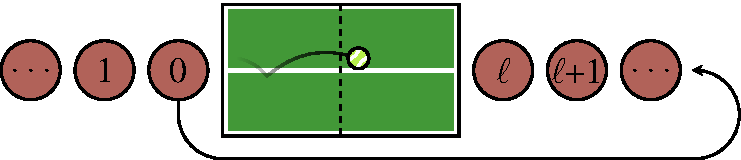
\includegraphics[width=0.75\textwidth]{slide.pdf}
\end{frame}

\begin{frame}
	\frametitle{\problemtitle}
	  \centering
	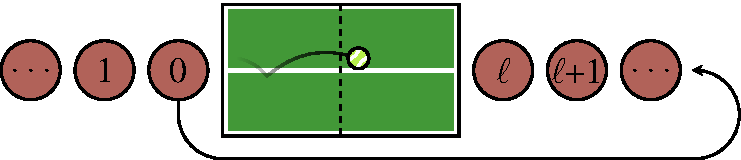
\includegraphics[width=0.5\textwidth]{slide.pdf}
%	Enumerate players: $\ell - 1,\; \ell - 2, \; \ldots, \;1, \; 0 \qquad \qquad \ell, \; \ell + 1,\; \ldots \;, \; \ell + r - 1$
	\begin{block}{Observations}
		\begin{itemize}
			\item Player $i$ on the left may face player $i + \ell$ and player $i + \ell - 1$ ($\bmod n$)
			\item Player $i$ on the right may face player $i + r$ and player $i + r + 1$ ($\bmod n$)
			\pause 
%			\item Case: player $i$ has the ball
%			\begin{itemize}
%				\item Player $i$ on the left $\Rightarrow$ faces player $i + \ell \bmod n$
%				\item Player $i$ on the right $\Rightarrow$ faces player $i + r + 1 \bmod n$
%			\end{itemize}
%			\pause
%			\item Case: player $i$ is in front without ball
%			\begin{itemize}
%				\item Player $i$ on the right faces player $i - \ell - 1 \bmod n$
%				\item Player $i$ on the left faces player $i - r \bmod n$
%			\end{itemize}
%			\pause
			\item Each player faces $\leq 4$ different players $\Longrightarrow$ $\leq 2n$ pairs in total with $n$ players
			\pause
			\item Some of the four indices may be equal $\Longrightarrow$ fewer opponents per player in this case
		\end{itemize}

		% \end{itemize}
	\end{block}
	\pause
	\begin{block}{Solution}
		\begin{itemize}
			\item If $r = \ell - 1$, then each player faces two different players $\Longrightarrow$ $n$ pairs
			\pause
			\item If $r = \ell$ or $r = \ell - 2$, then each player faces three different players $\Longrightarrow$ $n + \frac{n}{2}$ pairs

			\pause
			\item Else $2n$ pairs
		\end{itemize}
	\end{block}
	% \stats
\end{frame}
